\documentclass{sigchi}

% Remove or comment out these two lines for final version
\toappear{ Permission to make digital or hard copies of all or part of
  this work for personal or classroom use is granted without fee
  provided that copies are not made or distributed for profit or
  commercial advantage and that copies bear this notice and the full
  citation on the first page. To copy otherwise, or republish, to post
  on servers or to redistribute to lists, requires prior specific
  permission and/or a fee.

Gamification'13, October 2-4, 2013, Stratford, ON, Canada.

Copyright 2013 ACM 978-1-XXXX-XXXX-X/XX/XX...\$10.00.
}

\pagenumbering{arabic}% Arabic page numbers for submission. 

% Use \toappear{...} to override the default ACM copyright statement (e.g. for preprints).

% Load basic packages
\usepackage{balance}  % to better equalize the last page
\usepackage{graphicx} % for EPS, load graphicx instead
\usepackage{times}    % comment if you want LaTeX's default font
\usepackage{url}      % llt: nicely formatted URLs
\usepackage{paralist} % compact lists


\usepackage{subfigure}
\graphicspath{{figures/}}

% llt: Define a global style for URLs, rather that the default one
\makeatletter
\def\url@leostyle{%
  \@ifundefined{selectfont}{\def\UrlFont{\sf}}{\def\UrlFont{\small\bf\ttfamily}}}
\makeatother
\urlstyle{leo}

% To make various LaTeX processors do the right thing with page size.
\def\pprw{8.5in}
\def\pprh{11in}
\special{papersize=\pprw,\pprh}
\setlength{\paperwidth}{\pprw}
\setlength{\paperheight}{\pprh}
\setlength{\pdfpagewidth}{\pprw}
\setlength{\pdfpageheight}{\pprh}

%% Puts space after macros, unless followed by punctuation
\usepackage{xspace}

%%% Personal macros
%% Tired of typing CO2 so many times, requires xspace package
\newcommand{\COtwo}{CO\ensuremath{_2}\xspace}
%% Hawai`i with okina
\newcommand{\Hawaii}{Hawai`i\xspace}
%% Hawai`ian with okina
\newcommand{\Hawaiian}{Hawai`ian\xspace}
%% Manoa with kahako
\newcommand{\Manoa}{M\=anoa\xspace}

% Make sure hyperref comes last of your loaded packages, 
% to give it a fighting chance of not being over-written, 
% since its job is to redefine many LaTeX commands.
\usepackage[dvips]{hyperref}
\hypersetup{
pdftitle={SGSEAM: Assessing Serious Game Frameworks from a Stakeholder Experience Perspective},
pdfauthor={LaTeX},
pdfkeywords={SIGCHI, proceedings, archival format},
bookmarksnumbered,
pdfstartview={FitH},
colorlinks,
citecolor=black,
filecolor=black,
linkcolor=black,
urlcolor=black,
breaklinks=true,
}

%% Make links to captions point to the figure, not just the caption at bottom
\usepackage[all]{hypcap}

% create a shortcut to typeset table headings
\newcommand\tabhead[1]{\small\textbf{#1}}

%% Since I'm using the LaTeX Makefile that uses dvips, I need this
%% package to make URLs break nicely
\usepackage{breakurl}

% End of preamble. Here it comes the document.
\begin{document}

\title{SGSEAM: Assessing Serious Game Frameworks\\ from a Stakeholder Experience Perspective}

% Note that submissions are blind, so author information should be omitted
%\numberofauthors{5}
%\author{
%  \alignauthor Yongwen Xu, Philip M. Johnson, Carleton A. Moore, Robert S. Brewer, Jordan Takayama\\
%    \affaddr{Department of Information and Computer Sciences}\\
%    \affaddr{University of Hawaii at Manoa}\\
%    \affaddr{Honolulu, HI, USA}\\
%    \email{\{yxu, johnson, cmoore, rbrewer, jktakaya\}@hawaii.edu}\\
%}

\maketitle

\begin{abstract}
% 150 words max
Assessment of serious game frameworks is emerging as an important area of research.
This paper describes an assessment mechanism called the Serious Game Stakeholder Experience
Assessment Method (SGSEAM). SGSEAM is designed to provide detailed insights into the strengths
and shortcomings of serious game frameworks through a stakeholder perspective based approach.

In this paper, we report on the use of SGSEAM to assess Makahiki, an open source serious game
framework for sustainability.  Makahiki facilitates the development of serious games for the
purpose of education and behavioral change regarding energy and water consumption. Our results
provide useful insights into both Makahiki as a serious game framework and SGSEAM as an
assessment method.
\end{abstract}

\keywords{
	serious games; framework assessment; sustainability
}

\category {H.5.m.} {Information Interfaces and Presentation (e.g., HCI)} {Miscellaneous} {K.8.0.} {Personal Computing} {Games}

%\\
%\textcolor{red}{See: \url{http://www.acm.org/about/class/1998/}
%for more information and the full list of ACM classifiers and descriptors. 
%Mandatory section: On the submission page
%only the classifiers' letter-number combination will need to be entered.}


\terms{
	Serious Game; Assessment; Game Design; Case study.
}

\section{Introduction}

Serious games (games with additional goals beyond just entertainment) have been a topic
of academic research for decades~\cite{Zyda2005}. Such games show great potential as
interactive media that provide engaging interfaces in various serious
contexts~\cite{mcgonigal2011reality,reeves2009total}. The recent phenomenon of
gamification~\cite{Deterding2011mt} also calls for game-related research in areas beyond
traditional entertainment purposes.

One fundamental question in evaluating a serious game is the extent to which the
game achieves its ``serious'' purpose.  This is quite different from 
traditional entertainment games, in which evaluation focuses on usability or
playability~\cite{song2007new}. In the field of serious games, there is an increasing
focus on the methodology of research and evaluation~\cite{Mayer2012233}. De Freitas and
Oliver describe a four dimensional framework~\cite{de2006can} for evaluating an
educational game, consisting of: the context, the pedagogy, the representation, and the
learner (or player). Harteveld proposes an alternative approach called ``Triadic Game
Evaluation''~\cite{harteveld2010triadic}, consisting of three perspectives: Reality,
Meaning, and Play.

The above approaches focus on evaluation of a single game, as opposed to a game {\em
  framework}. Game frameworks (also known as game engines) are ``comprised of a collection
of different tools, utilities, and interfaces that hide the low-level details of the
various tasks that make up a game''~\cite{sherrod2006ultimate}. One of the benefits of
using a serious game framework is that, if correctly designed, it will provide useful and
reusable ``building blocks'' with which to develop a variety of serious games.  These
building blocks enable the serious game developer to focus more time and thought on
content and results instead of on infrastructure. Yet how are we to know if a serious
game framework has been ``correctly designed''?

Upon review of the literature, we found little prior work concerning formal assessment for
the particular needs of serious game frameworks. To help answer this question, this paper
proposes a method for assessing serious game frameworks, called the Serious Game Stakeholder
Experience Assessment Method (SGSEAM). In a nutshell, SGSEAM (pronounced "sig-seam")
identifies the most important stakeholders of a
serious game framework and provides a method for gaining insight into the strengths
and shortcomings of the framework with respect to each stakeholders' needs. We consider
SGSEAM as an assessment method instead of an evaluation method. The main purpose of an
evaluation is to "determine the quality of a program by formulating a judgement"
\cite{hurteau2009legitimate}. An assessment, on the other hand, is nonjudgmental. SGSEAM does
not try to judge a framework according to a standard, instead, it is used to identify the major
strengths and shortcomings of a framework so that the community could benefit from the
assessment by learning from the strengths and improving the shortcomings.

In the next section, we describe SGSEAM in detail. We then describe our preliminary results
from the application of SGSEAM to Makahiki, a serious game framework for sustainability we
developed. We conclude with the insights this assessment process provides
for our own work on Makahiki, serious game design in general and
serious game framework assessment.

\section{Serious Game Stakeholder Experience Assessment Method (SGSEAM)}

The goal of SGSEAM is to identify (a) major strengths of a serious game
framework, which aids the community by indicating features of the framework to emulated, and
(b) major shortcomings of the framework, which aids the community by indicating features to avoid
and the developers of the framework by indicating the areas to improve on.

The approach that SGSEAM uses is to assess the experiences of various important stakeholders when
they interact with the serious game framework. In the full life cycle of a serious game framework
there are a great variety of potential stakeholders, including:

\begin{compactitem}
\item \emph{Players}: those who participate in the game produced by the framework.
\item \emph{System admins}: those who install and maintain the technological game infrastructure.
\item \emph{Game designers}: those who design the content and game mechanics.
\item \emph{Game managers}: those who manage the game during the period of game play.
\item \emph{Developers}: those who extend, enhance and debug the game framework.
\item \emph{Researchers}: those who are conducting research using the game framework.
\item \emph{Spectators}: those who do not participate in the game play
  but are interested in the game and the results of game play. 
\item \emph{Community partners}: those who partner with the game
  organizers to help run the game (such as coordinating real-world
  events as part of the game, providing support for energy data
  collection, etc) 
\item \emph{Funding organizations}: the organizations who provide
  funding for the game or game framework.
\end{compactitem}

The scope of SGSEAM is to assess serious game frameworks as software infrastructure. While
the overall success of a serious game depends on the individual success of all of these
stakeholders, SGSEAM does not address the spectator, community partner, and funding
organization stakeholders. These are important stakeholders but outside the scope of our
assessment. In the context of a serious game framework, SGSEAM focuses on players, system admins, game designers, developers and researchers.

The following sections describe the methodology used in SGSEAM, followed by the detailed
description of assessment methods for each identified stakeholder.

\subsection{Methodology}

Creswell \cite{creswell2003} categorizes research methods into three approaches:
quantitative, qualitative, and mixed methods, according to what knowledge claims are being made
and how knowledge is acquired. Quantitative method reflects a post-positivist paradigm where
hypotheses are specified {\em a priori} and tested by experimental design. Qualitative method
reflects a constructivist or participatory paradigm where knowledge would be acquired by
observation and open-ended design. SGSEAM employs the mixed methods approach which based on
pragmatic knowledge claims and assumption that collecting diverse types of data provides better
understanding of the research problem: assessing the strengths and shortcomings of a serious game
framework.

In SGSEAM, the concurrent triangulation strategy \cite{creswell2003} of the mixed method approach
is used.  Data collection and analysis involves both quantitative information (instrument and
analytical data recorded by the system such as website logs, interaction database, etc), as well
as qualitative information (interviews and questionnaire responses).

\subsection{Stakeholder Experience Assessment}

SGSEAM follows closely with the "Goal-Question-Metric" (GQM) approach \cite{caldiera1994goal} in
software engineering research. GQM defines a software  measurement model on three levels: a goal
of the measurement, a set of questions to assess the goal, and a set of metrics associated with
each question.

In SGSEAM, the assessment goals are the experiences of the identified stakeholders. For each
stakeholder, a set of questions is used to assess the strengths and shortcomings from the
stakeholder's perspective. For each question, a set of alternative assessment approaches is
proposed.

\autoref{fig:overview} provides an overview of the assessment method:

\begin{figure}[ht!]
  \centering
  \begin{tabular}{|c|c|c|}
    \hline
    \multicolumn{1}{|p{0.2\columnwidth}|}{\centering\tabhead{Stakeholder (Goal)}} &
    \multicolumn{1}{|p{0.35\columnwidth}|}{\centering\tabhead{Assessment question}} &
    \multicolumn{1}{|p{0.35\columnwidth}|}{\centering\tabhead{Assessment approaches}} \\
    \hline
    \multicolumn{1}{|p{0.2\columnwidth}|}{Players} &
    \multicolumn{1}{|p{0.35\columnwidth}|}{To what extent does the system affect players?
        To what extent does the system engage players?} &
    \multicolumn{1}{|p{0.35\columnwidth}|}{experimental study, interviews,
                engagement metrics} \\
    \hline
    \multicolumn{1}{|p{0.2\columnwidth}|}{System admins} &
    \multicolumn{1}{|p{0.35\columnwidth}|}{How easy is it to install and maintain the system?} &
    \multicolumn{1}{|p{0.35\columnwidth}|}{experimental study, interviews} \\
    \hline
    \multicolumn{1}{|p{0.2\columnwidth}|}{Game designer} &
    \multicolumn{1}{|p{0.35\columnwidth}|}{How easy is it to design a game?} &
    \multicolumn{1}{|p{0.35\columnwidth}|}{experimental study, system logs, interviews } \\
    \hline
    \multicolumn{1}{|p{0.2\columnwidth}|}{Game managers} &
    \multicolumn{1}{|p{0.35\columnwidth}|}{How easy is it to manage a game?} &
    \multicolumn{1}{|p{0.35\columnwidth}|}{experimental study, system logs, interviews} \\
    \hline
    \multicolumn{1}{|p{0.2\columnwidth}|}{Developers} &
    \multicolumn{1}{|p{0.35\columnwidth}|}{How easy is it to enhancing the system?} &
    \multicolumn{1}{|p{0.35\columnwidth}|}{experimental study interviews} \\
    \hline
    \multicolumn{1}{|p{0.2\columnwidth}|}{Researchers} &
    \multicolumn{1}{|p{0.35\columnwidth}|}{How easy is it to do research with the system?} &
    \multicolumn{1}{|p{0.35\columnwidth}|}{research outcome interviews} \\
    \hline
  \end{tabular}
  \caption{Overview of SGSEAM}
  \label{fig:overview}
\end{figure}

There are usually multiple assessment approaches for a specific question. Different assessment
approaches will have different levels of rigor. In experimental design terms, rigor refers to
external and internal validity. The details of the individual assessment approach for each
stakeholder are descried in the following sections. The assessment approaches for a question
can be additive. The more approaches applied, the higher confidence of the assessment.

\subsubsection{Player Assessment}

The goal of player assessment is to determine the effectiveness of the game
framework from player's perspective. It is essential that a game produced by a serious game
framework could achieve its intended "serious" purpose. The intended purposes of serious games are
always subject specific. For example, the desired effect of a serious game for
energy education and conservation is to increases players' energy literacy and
reduces their energy consumption during (and, hopefully, after) the game. A serious game for
language learning would have a very different desired effect.

Users of SGSEAM could use domain-specific questions to assess the desired effects of their
serious game. For illustration purpose, the following two questions are used to assess a serious
game for sustainability: (a) To what extent does the game increase player's literacy in
sustainability? (b) To what extent does the game produce positive player behavior change in
sustainability?

One approach to assess the question of the effect of literacy changes is a quasi-experimental
study. A set of literacy survey questionnaires are presented to a random selection of the players
before the game (pre-test). After the game ends, the same survey (post-test) is presented to the
players who responded the pre-test survey. These two set of survey response data are compared to
understand if the game has had an impact on literacy. The extent of players' sustainability
literacy change will indicate the degree of educational effectiveness of the serious game for
sustainability.

A pre-experimental study could be used to assess the question of the effect of
sustainability behavior changes. The resource (energy and/or water) consumption data during and
after the game are recorded (post-test). They are compared to the resource consumption baseline
established before the game (pre-test).

Another approach for effectiveness assessment is to interview players about their self-reported
behavior change. The combination of resource consumption changes and self-reported behavior changes
can be combined to assess the degree of behavior effectiveness of the serious game for
sustainability.

In addition to the domain-specific goals of serious games, SGSEAM assesses a common
aspect of serious games, player engagement, to address the question of "To what extent does the
game engage players?"

Player engagement is an important measure for understanding the effectiveness of a serious game.
By investigating the degree of engagement, we can determine to what extent individuals are
participating in the game, as well as to what extent the community population is participating in
the game.

Engagement has a subtle relationship to the overall effectiveness of a serious game. It is
possible for the game to be played by only a subset of the target population, but
have an impact on those not playing by virtue of their contacts with players. Gaining
better insight into this effect is an area of active study for us. 

To obtain engagement data, SGSEAM analyzes the following measures
based upon system log data provided by the framework.

\begin{compactitem}
\item participation rate
\item number of players per day
\item play time of a player per day
\item submissions of all player per day
\item social interaction of all player per day
\item website errors per day
\end{compactitem}

The participation rate measures the percentage of users who used the game based on the total
eligible players. In the serious game context, it indicates the level of involvement or awareness
of the serious matters. The number of players and play time per day measure how frequently the
players interact with the game. The submissions per day measures the rate of serious game
specific activities (online or real world) that players completed, while the social interaction
per day measures the rate of social interactions happened in the game between the players. At
last, the website errors per day measures the rate of errors encountered by the players while
using the game website. In general, with the opposite of website error measurement, the higher
value these measurements are, the higher engagement level the game has.

\subsubsection{System Admin Assessment}

System administrators are responsible for installing and maintaining the software infrastructure
for the game. Their tasks include the framework and dependency installation, maintain the database, backups, and so forth.

One approach to assess the question of how easy it is to install and maintain the system is to use
an experimental study. A group of system admins is asked to install the system, record the time
spent and problem encountered as they complete each step. The qualitative data (i.e., the
descriptive problems reported by the participants of the study) will need to be categorized and
coded. The assessor will triangulate the reported time data and the problem categories to identify
the area of strength (less time spent) and weakness (problems and difficulties).

Another approach is a post-hoc interview. The system admin(s) are asked about their experience
after the installation. The interview includes the following questions:

\begin{compactitem}
\item How much time did you require to install the system and the dependencies?
\item How much time did you require to maintain the system?
\item What problems did you encounter?
\item Did you find it difficult to admin the system? What was difficult?
\end{compactitem}

After the interview data is acquired, the assessor will perform qualitative data
analysis, which involves transcribing (if the interview data is in audio format),
categorizing and coding the description of reported problems or difficulties.

The level of confidence of the above two assessment approaches varies. The experimental study
approach is more rigor because of the generality achieved from the larger population of
participants under study. The data collected during the step by step experimental study is more
accurate than the one collected in the post-hoc interview.

\subsubsection{Game Designer Assessment}

A game designer uses the serious game framework to design and create a serious game.
A serious game framework always provides certain tools or interfaces to game designers
with the hope that these will simplify the design of a game. Such tools might involve
configuring global settings for the game, such as how long will the game run, who are the
players, and how to design individual game elements.

SGSEAM assesses the game designer stakeholder by addressing the following two questions: (a) How
much time is required to design an instance of a serious game using the framework? and (b) How
many, and how problematic are the errors that designers encounter during the design process?

There are also three approaches for game designer assessment. One is a experimental study, where a
goup of participants is asked to use the system to perform a same set of design tasks. The time
spent and problems encountered are recorded for each tasks. The assessor will triangulate the
reported time data and the problem categories to identify the strengths and weaknesses.

A second approach is to interview the designer(s) after they had completed the design.
The following questions will be asked:
\begin{compactitem}
\item How much time did you spend to complete each design task?
\item What problems did you encounter?
\item Did you find it difficult to configure? What was difficult?
\item Did you find it difficult to design a specific game? Which one, and what was difficult?
\end{compactitem}

The interview data will be transcribed (if audio recording), categorized and coded to identify the
strengths and weaknesses.

A third approach is to collect the system log data related to the game designing tasks. When
available, the time spent and error encountered can be queried from the system logs. Although these
system generated data might be easier to gather in some systems, it might not provide the same
depths or insights than the other two approaches where the experiences are provided by the
participants directly. On the other hand, these system data can be supplemental to the other
approaches. They could be correlated with the data gathered from the other assessment approaches
 to increase the confident of the assessment.

\subsubsection{Game Manager Assessment}

A game manager uses the serious game framework to manage the serious game that the game
designers created. It is possible that a game manager is also the game designer.
Serious game frameworks normally provide certain interfaces for the managers to manage the
game. This may involve managing player submissions, monitoring the game state, entering
manual resource data, notifying winners of the game, etc.

SGSEAM assesses the game manager stakeholder with the following questions: (a) How much time is
required to manage an instance of a serious game using the framework? and (b) How many,
and how problematic are the errors that managers encounter during the design process?

Similar to the assessment of game designer experience, SGSEAM proposes three approaches. The
experimental study approach gather data from a group of participants about the time spent and
problems encountered for each task of managing the serious game. The post-hoc interview approach
gather data from the game manger(s) by asking the following questions:

\begin{compactitem}
\item How much time did you spend to complete each managing task?
\item What problems did you encounter?
\item Did you find it difficult to manage? What was difficult?
\end{compactitem}

\subsubsection{Developer Assessment}

The developer stakeholder is different from the game designer stakeholder, in that the
game designer stakeholder tailors the framework without requiring any software
development, while the Developer stakeholder enhances, corrects, and extends the system by
manipulating code. 

To investigate how easy it is to understand, extend, and debug a serious game
framework from a developer's perspective, SGSEAM assesses how much time it takes to develop an
enhancement to the game framework, and how many errors are encountered
during the process.

The experimental study assessment approach asks a group of developers to develop a same set of
enhancements to the system, and ask them to record the time spent to develop and problems
encountered.

A second assessment approach is accomplished by interviewing the developer(s) to
answer the following questions:

\begin{compactitem}
\item How much time did you spend developing and debugging an
  enhancement to the game framework?
\item What problem(s) did you encounter?
\item Did you find it difficult to understand, extend and debug the
  system? What was difficult?
\end{compactitem}

Similarly, the descriptive data will be categorized and coded. The time data will be correlated to the problem data to identify the areas of strength and weaknesss.

\subsubsection{Researcher Assessment}

Finally, the researcher stakeholder is the one who uses the serious game framework to
investigate questions about serious games, human computer interaction, etc.

To investigate how effective it is to do research with the system, SGSEAM proposes two assessment
approaches. One is to assess the research outcomes to identify the numbers of research
accomplishments with the help of the system, for example, the number of research papers published.

Another approach is to interview researcher to answer the following questions:
\begin{compactitem}
\item How much time did you spend to collect the research data for a
  specific topic?
\item Is the data you get from the system useful?
\item What problems did you encounter when collecting the data?
\item Did you find it difficult to collect data from the system?
  What was difficult?
\end{compactitem}

\section{Case Study of Makahiki}

This section presents a case study of how we applied SGSEAM to assess Makahiki, an open source serious
game framework for sustainability. 

\subsection{Makahiki in Brief}

Sustainability education and conservation have become an international imperative due to the
rising cost of energy and increasing scarcity of natural resources. Over the past decade, energy
and water challenges have become focal points for sustainability efforts at both university and
industry campuses. For example, there are more than 160 college residence hall energy
competitions taking place or being planned for the 2010--2011 academic year in North America~\cite{Hodge2010} to engaging students in sustainability issues.

We developed Makahiki \cite{csdl2-12-06} to facilitate the creation of sustainability challenges by
different organizations. It is an innovative serious game framework for sustainability with
the purpose of education and behavioral change regarding energy and water consumption.
Its extensible software system includes a variety of common services such as authentication; game mechanics such as leaderboards, points, and badges; a variety of built-in games and
content focused on sustainability; a responsive user interface; cloud-based deployment;
and the ability to customize the game to the needs of individual organizations.
Figure \ref{fig:Makahiki-Home-Page} illustrates a home page implemented using Makahiki.

\begin{figure}[ht!]
  \center
  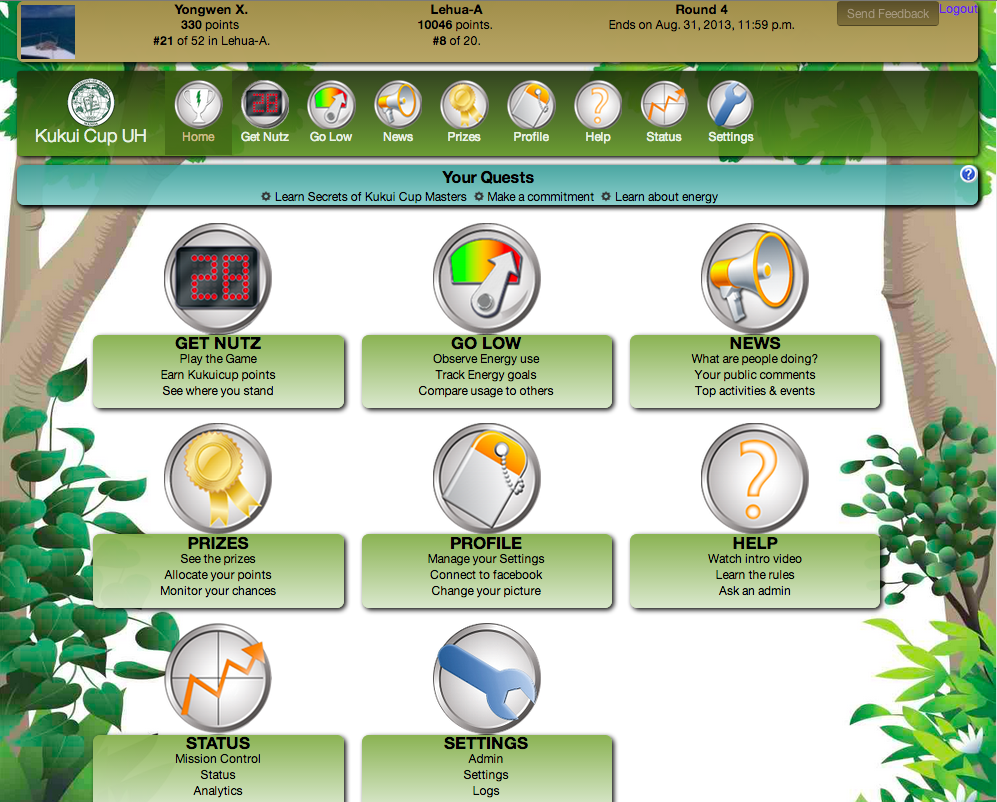
\includegraphics[width=\columnwidth]{kukuicup-home}
  \caption{Makahiki Game Instance}
  \label{fig:Makahiki-Home-Page}
\end{figure}

Makahiki consists of a library of
pre-built game ``widgets'' that implement a variety of game mechanics.
Using the widgets, an organization can create a custom sustainability
challenge in which players can compete individually or in teams to
earn points and reduce consumption of resources such as water or energy.
\autoref{fig:makahiki-architecture} illustrates the architecture of
Makahiki.

\begin{figure}[ht!]
  \center
  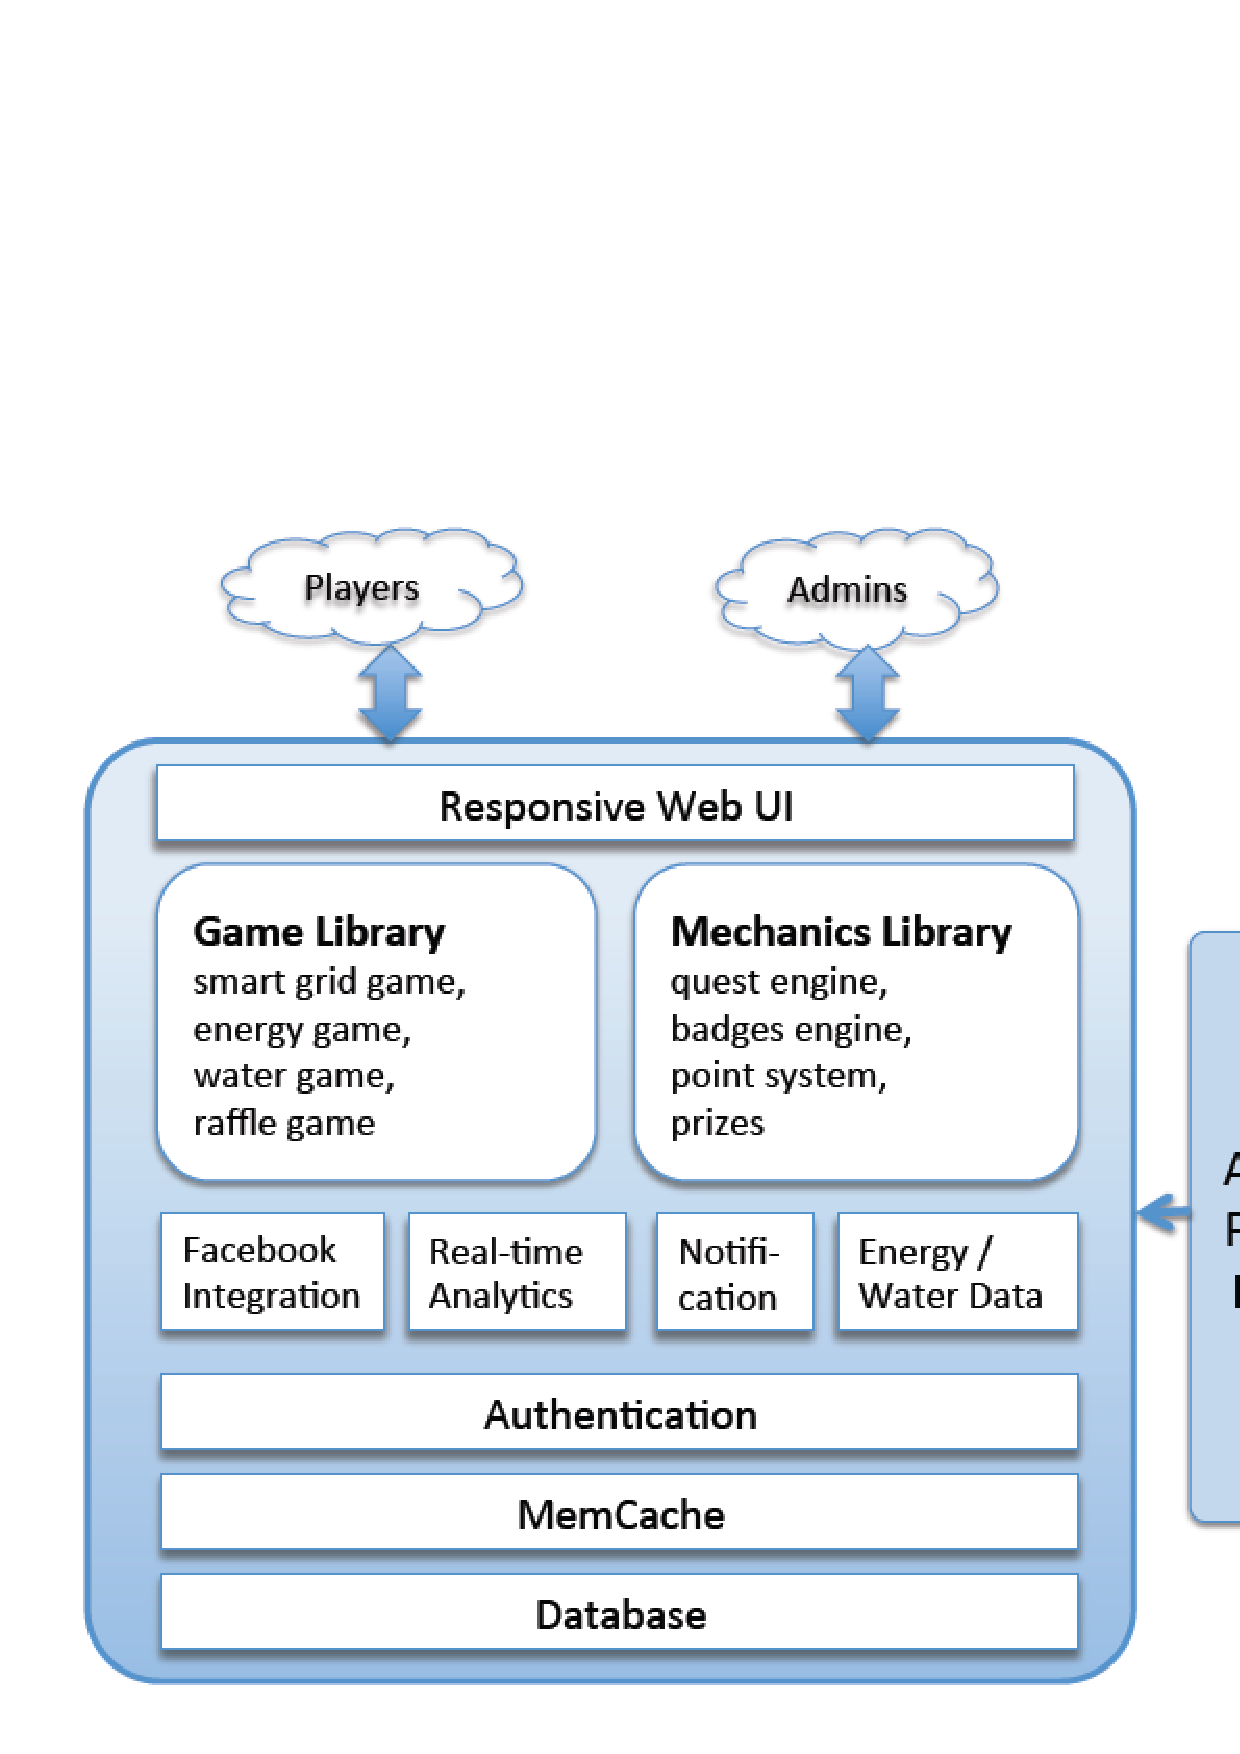
\includegraphics[width=\columnwidth]{makahiki-system-architecture}
  \caption{Architecture of Makahiki}
  \label{fig:makahiki-architecture}
\end{figure}

\subsection{Experiences with Makahiki}

We have used Makahiki to create four different Kukui Cup Energy Challenges. Kukui Cup
Energy challenges were held at the University of Hawaii (UH) in 2011 and 2012 for over
1,000 first year students living in the residence halls. Hawaii Pacific University (HPU)
held a Kukui Cup Energy challenge in Fall 2012 for about 200 students. An international
organization called the East-West Center (EWC) held a Kukui Cup Energy and Water challenge
for approximately 600 international residents living in their residence halls. Since the
halls did not have internet-enabled meters, resource consumption data had to be entered by
the game managers manually.

The successful creation of serious game challenges by three different organizations
provides evidence that Makahiki can be successfully tailored
to the needs of different organizations. First, UH and HPU used different metering
infrastructure, and EWC collected their resource data manually.  Second, while UH and HPU
challenges involved only energy consumption data, the EWC challenge involved both energy
and water consumption data. Third, the IT infrastructure at UH and HPU provided
authentication services using CAS (Central Authentication Service) and LDAP, while EWC
used the built-in Django authentication.  Fourth, the user interface was customized to
``brand'' each challenge with the logo, thematic elements, and the education contents of
the sponsoring organizations.

Besides the real world usage of Makahiki in the series of Kukui Cup challenges, we
performed in-lab assessment experiments in 2013. Makahiki was used in a serious game
development course in Spring semester of 2013 at the Information and Computer Sciences
Department of the University of Hawaii at Manoa. There were a total of 8 students who
participated in the experiments.  The participants were either senior undergraduates or
graduate students majoring in Computer Science. During the course, the students installed
Makahiki, configured and designed a serious game instance with Makahiki, and finally
developed an enhancement to the Makahiki framework. We asked the students taking the
course to voluntarily participate in the assessment experiments of Makahiki, using SGSEAM.

\subsection{Assessing Makahiki using SGSEAM}

\subsubsection{Makahiki Player Assessment}

We applyed SGSEAM to assess player effectiveness during the 2011 Kukui Cup Challenge at
the University of Hawaii at Manoa, a serious game implemented using the Makahiki
framework. There were over 1000 eligible players for this challenge, who were mostly first
year college students living in the resident halls. The challenge lasted for 3 weeks.
Makahiki recorded detailed logging data from every interaction between the players and the
website.

To assess the effectiveness of the framework for designing games that improve player literacy in sustainability, we
conducted two energy literacy surveys, one before the challenge (pre-game) and one after
the challenge (post-game). 24 players completed both surveys. Out of the total 19 energy
literacy questions, the average number of questions answered correctly is 7.54 before the
challenge, and 8.96 after the challenge. This result indicates an 18\% improvement on the
energy literacy.  We also surveyed non-players as a control condition, and found that
their literacy did not change, indicating that the improvement in player literacy was
indeed due to the game. 

To assess the effectiveness of the framework for designing games that produce positive change in sustainability
behaviors, we recorded and analyzed energy consumption data before, during and after the
challenge.  Before the challenge, an energy usage baseline was established. During the
challenge, compared to the baseline, 12 out of the total 20 teams reduced their energy
consumption, with the highest reduction of 16.1\%. However, 3 teams actually increased
their energy consumption, with the highest increase of 11.7\%. Overall, the average
reduction of the 20 teams was very low---approximately 2\%.

To assess player engagement of the game, we calculated a variety of engagement
metrics. The results are shown in \autoref{fig:makahiki-engagement}:

\begin{figure}[ht!]
  \centering
  \begin{tabular}{|c|c|c|c}
    \hline
    \multicolumn{1}{|p{0.5\columnwidth}|}{\centering\tabhead{Measurement}} &
    \multicolumn{1}{|p{0.1\columnwidth}|}{\centering\tabhead{MIN}} &
    \multicolumn{1}{|p{0.1\columnwidth}|}{\centering\tabhead{AVG}} &
    \multicolumn{1}{|p{0.1\columnwidth}|}{\centering\tabhead{MAX}} \\
    \hline
    \multicolumn{1}{|p{0.5\columnwidth}|}{Participation rate} &
    \multicolumn{1}{|p{0.1\columnwidth}|}{13\%} &
    \multicolumn{1}{|p{0.1\columnwidth}|}{37\%} &
    \multicolumn{1}{|p{0.1\columnwidth}|}{74\%} \\
    \hline
    \multicolumn{1}{|p{0.5\columnwidth}|}{Number of players per day} &
    \multicolumn{1}{|p{0.1\columnwidth}|}{43} &
    \multicolumn{1}{|p{0.1\columnwidth}|}{85} &
    \multicolumn{1}{|p{0.1\columnwidth}|}{147} \\
    \hline
    \multicolumn{1}{|p{0.5\columnwidth}|}{Play time per day} &
    \multicolumn{1}{|p{0.1\columnwidth}|}{1 min} &
    \multicolumn{1}{|p{0.1\columnwidth}|}{27.7 mins} &
    \multicolumn{1}{|p{0.1\columnwidth}|}{8.5 hours} \\
    \hline
    \multicolumn{1}{|p{0.5\columnwidth}|}{submissions per day} &
    \multicolumn{1}{|p{0.1\columnwidth}|}{32} &
    \multicolumn{1}{|p{0.1\columnwidth}|}{266} &
    \multicolumn{1}{|p{0.1\columnwidth}|}{1110} \\
    \hline
    \multicolumn{1}{|p{0.5\columnwidth}|}{social interactions per day} &
    \multicolumn{1}{|p{0.1\columnwidth}|}{51} &
    \multicolumn{1}{|p{0.1\columnwidth}|}{208} &
    \multicolumn{1}{|p{0.1\columnwidth}|}{468} \\
    \hline
    \multicolumn{1}{|p{0.5\columnwidth}|}{website errors per day} &
    \multicolumn{1}{|p{0.1\columnwidth}|}{0} &
    \multicolumn{1}{|p{0.1\columnwidth}|}{0.6} &
    \multicolumn{1}{|p{0.1\columnwidth}|}{4} \\
    \hline
  \end{tabular}
  \caption{Makahiki Engagement Metrics}
  \label{fig:makahiki-engagement}
\end{figure}

The participation rate of this challenge is 37\%, which is good compared to other
sustainability challenges. Over the course of the challenge, an average player spent about
27.7 minutes per day on the website. One player spent 8.5 hours on one day. There were an
average of 266 activity submissions and 208 social interactions between players per day.

In summary, SGSEAM indicates that Makahiki can be successful in achieving
player engagement and literacy improvement. SGSEAM could not provide evidence of positive change in
behavior.

\subsubsection{Makahiki System Admin Assessment}

System admin assessment was done using an in-lab experiment.  Students in
a serious game class were tasked with installing the Makahiki system into their local
computers. In order to understand how much time it takes to install Makahiki and what
problems might be encountered, we designed a Google Form explaining the steps required to
install Makahiki. We asked the students to record the time they spent completing each step
and the problems they encountered. We also asked the students to provide feedback about
their installation experiences in the form of blog posts. \cite{csdl2-13-04} describes in detailed
the Google Form that is used in this assessment.

The results from the Google Form responses show that the average total time to successfully install
Makahiki was 1.4 hours, with a maximum time of 2 hours and the minimum time of 0.9 hour.
\autoref{fig:install-time} shows the average time for each installation step.

\begin{figure}[ht!]
  \center
  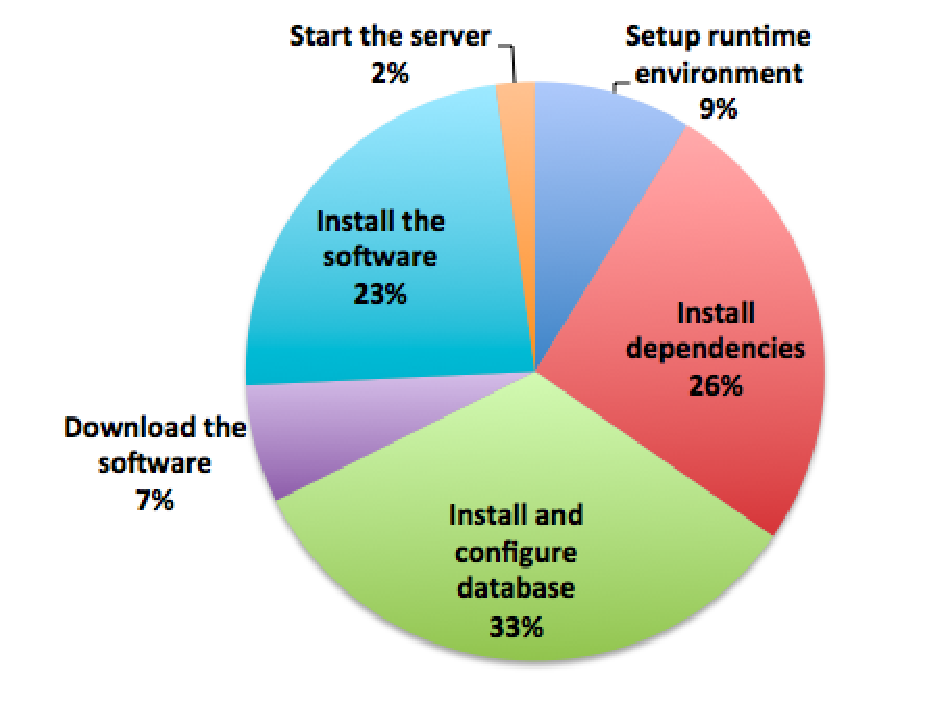
\includegraphics[width=0.8\columnwidth]{install-time}
  \caption{Average time for installation step}
  \label{fig:install-time}
\end{figure}

We coded and categorized the descriptive problems reported by the students in both the Google Form
and their blog posts. \autoref{fig:makahiki-install} shows the result of the analysis from
the feedback of the 8 students that participated in the experiment.

\begin{figure}[ht!]
  \centering
  \begin{tabular}{|c|c|}
    \hline
    \multicolumn{1}{|p{0.7\columnwidth}|}{\centering\tabhead{Problem encountered}} &
    \multicolumn{1}{|p{0.2\columnwidth}|}{\centering\tabhead{Number of participants}} \\
    \hline
    \multicolumn{1}{|p{0.7\columnwidth}|}{Cannot find configuration file to edit during database installation } &
    \multicolumn{1}{|p{0.2\columnwidth}|}{4} \\
    \hline
    \multicolumn{1}{|p{0.7\columnwidth}|}{Documentation of install script is confusing about creation of the DB user} &
    \multicolumn{1}{|p{0.2\columnwidth}|}{2} \\
    \hline
    \multicolumn{1}{|p{0.7\columnwidth}|}{More parts of installation could be covered by install script} &
    \multicolumn{1}{|p{0.2\columnwidth}|}{2} \\
    \hline
  \end{tabular}
  \caption{Makahiki Installation Analysis (n=8)}
  \label{fig:makahiki-install}
\end{figure}


From the above analysis, we identified that the ``Install and configure database'' step has the
longest average time. It is also has the most participant reported problems. This reflects the issues
encountered by students during the configuration process. This assessment determines the areas for future
improvement are (1) to improve documentation on DB installation, and (2) to improve the install script to automate
more installation tasks.

In summary, SGSEAM identified database installation as a weak point in
installation.  Otherwise, SGSEAM indicates generally positive results regarding
Makahiki with respect to installation. 

\subsubsection{Makahiki Game Designer Assessment}

We also used the in-lab experiment to assess the game
designer experience of Makahiki. One of the class assignments for the students in the
experiment was to design a serious game using the Makahiki framework. We asked the students
to follow specific design steps and record the time required and any problems encountered during
their design process, using a Google Form similar to the one used for the system admin
assessment. In addition, students were asked to provide feedback about their
design experiences in the form of blog posts. \cite{csdl2-13-04} describes in detailed
the Google Form that is used in this assessment.

The game designer assessment was generalized into 7 tasks corresponding to
distinct types of administrative tasks and game design planning. The time for each task is
calculated from the Google Form results.  The most time consuming task
 is "Smart Grid Game Design", which took average 107.9 minutes (56\% of total time) to complete,
 while the least time
  consuming tasks is "Raffle Game Design", which took average 7.9 minutes (7\% of total time)
  to complete.

\autoref{fig:design-time} shows the average time for each design tasks:

\begin{figure}[ht!]
  \center
  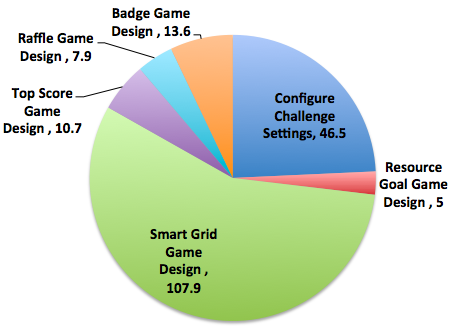
\includegraphics[width=0.8\columnwidth]{design-time}
  \caption{Average time for design tasks}
  \label{fig:design-time}
\end{figure}

 We aggregated the problems reported in the feedback of the 7 students that participated in the experiment.
\autoref{fig:makahiki-game-design} shows the result of the analysis:

\begin{figure}[ht!]
  \centering
  \begin{tabular}{|c|c|c|}
    \hline
    \multicolumn{1}{|p{0.7\columnwidth}|}{\centering\tabhead{Problem encountered}} &
    \multicolumn{1}{|p{0.2\columnwidth}|}{\centering\tabhead{Number of participants}} \\
    \hline
    \multicolumn{1}{|p{0.7\columnwidth}|}{Difficulty in understanding predicate system and unlock condition} &
    \multicolumn{1}{|p{0.2\columnwidth}|}{7} \\
    \hline
    \multicolumn{1}{|p{0.7\columnwidth}|}{A bug that prevented users with usernames
containing capital letters from logging in} &
    \multicolumn{1}{|p{0.2\columnwidth}|}{2} \\
    \hline
    \multicolumn{1}{|p{0.7\columnwidth}|}{A bug in the processing of Ajax queries} &
    \multicolumn{1}{|p{0.2\columnwidth}|}{1} \\
    \hline
    \multicolumn{1}{|p{0.7\columnwidth}|}{Difficulty in generating event attendance codes for game activities} &
    \multicolumn{1}{|p{0.2\columnwidth}|}{1} \\
    \hline
  \end{tabular}
  \caption{Makahiki Game Design Analysis, (n=8)}
  \label{fig:makahiki-game-design}
\end{figure}

In summary, SGSEAM revealed two shortcomings with Makahiki configuration: ``Smart
Grid Game Design'' and ``Configure Challenge Settings''. Issues encountered in ``Smart Grid Game
Design'' included 1) difficulty and lack of documentation on the predicate system used to define dependencies
between game activities, and 2) difficulty in generating event attendance codes for game activities.
Issues encountered in ``Configure Challenge Settings'' included 1) a bug in the processing of Ajax queries
caused by consecutive clicks on the same interface button, and 2) a bug that prevented users with username
containing capital letters from logging in.

\subsubsection{Makahiki Game Manager Assessment}

We used the 2012 Kukui Cup Challenge at the Hawaii Pacific University (HPU) to assess
the game manager experience of Makahiki. We interviewed the
game manager of the HPU Kukui Cup challenge, who is also the game designer of the challenge.
We asked him about his game management experiences using the Makahiki admin
interface. The interview questions are outlined in the game manager section of the SGSEAM.

The interview took place after the challenge and was audio-recorded. We transcribed the
audio recording. The data shows that the game management interface was easy for him to use.
He made sure that player submissions were either approved or rejected
within 12 hours. He also discovered a useful feature in the approval interface without
help from the Makahiki support team. The only problem he reported was that after the
competition ended, he discovered that some of the analytics data disappeared. This was
identified by the Makahiki development team as a software bug and has since been fixed.

In summary, SGSEAM uncovered few problems with Makahiki game management using the interview
approach. We realized that the confident level of this assessment approach is low because of
 availability of only one data point. An experimental study approach or perform interviews to
multiple game managers will increase the confidence level of the assessment.

\subsubsection{Makahiki Developer Assessment}

We assessed developer experience using an in-lab experiment. One of the class assignments
for the students in the experiment was to develop an enhancement to Makahiki.  This
involved setting up a development environment, following the tutorial to create a ``Hello
world'' widget using Makahiki, and finally, developing an enhancement to extend the
functionality of Makahiki.

The students were asked to submit their development source code to the
public source code repository (GitHub) and write a blog post to
discuss their efforts to complete the development activity.

All 8 students reported that the first task of creating the simple ``Hello world'' widget
was easy, while the enhancement development was hard. Only one student successfully
completed all 5 required features, while the rest successfully completed 1 or 2
features. The main problem students reported was the lack of documentation for the
development libraries. One student stated in his blog that he decided to choose Makahiki
framework to develop his own serious game because of Makahiki's features and possibility
of reducing development effort by using the framework.

In summary, SGSEAM reveals significant problems with developer efficiency.
Analysis is still ongoing regarding the specific causes of problems and how best to
address them.

\subsubsection{Makahiki Researcher Assessment}

Several researchers had used and are currently using Makahiki to perform
research in the areas of energy and sustainability behavior change. We assessed the effectiveness
of research experiences by identifying their research outcomes generated from the usage of Makahiki.
The outcomes of these research include: a) Five research papers published in international
conferences, b) One Ph.d dissertation, c) Five internal tech reports, d) Nine presentations.

In summary, SGSEAM provides a way to identify the effectiveness of Makahiki from researcher's
perspective. Assessment is ongoing to use the interview approach to understand how easy it is for
a researcher to perform research using Makahikiki.

\section{Conclusions}

We have developed a serious game framework assessment method called Serious Game
Stakeholder Experience Assessment Method (SGSEAM). SGSEAM assesses serious game
frameworks from the perspective of the following stakeholders' experiences: players
, system administrators, game designers, game managers, developers, and researchers.

These experiences are assessed qualitatively and quantitatively to identify the strengths and
 shortcomings of a serious game framework.

We applied SGSEAM to Makahiki. The results of the assessment show both strengths and
weaknesses in this framework.  Most importantly, the assessment has provided actionable
insight into how to improve the framework for system administrators, developers, and game
designers.  We now understand Makahiki far better than we did before the application of
SGSEAM.

Our use of SGSEAM also reveals concerns with the assessment method itself.  For certain
stakeholders, we took advantage of a course on serious game design to obtain fairly
detailed quantitative data about, for example, game design assessment.  While we feel
confident of these results, the effort required to collect the data was substantial.  On
the other hand, for other stakeholders such as game managers, we only had access to a
single person who could provide insight from that perspective.  While easier to collect,
the small sample size limits our confident in the data.  We are considering ways to
augment the method with a ``confidence'' value that helps others better interpret the
findings.  We also hope to apply SGSEAM to a different serious game framework in order to
gain additional insights into the strengths and limitations of this approach.

\section{Acknowledgments}
Omitted from review version.

%\textbf{Don't forget
%to acknowledge funding sources as well}, so you don't wind up
%having to correct it later.

% Balancing columns in a ref list is a bit of a pain because you
% either use a hack like flushend or balance, or manually insert
% a column break.  http://www.tex.ac.uk/cgi-bin/texfaq2html?label=balance
% multicols doesn't work because we're already in two-column mode,
% and flushend isn't awesome, so I choose balance.  See this
% for more info: http://cs.brown.edu/system/software/latex/doc/balance.pdf
%
% Note that in a perfect world balance wants to be in the first
% column of the last page.
%
% If balance doesn't work for you, you can remove that and
% hard-code a column break into the bbl file right before you
% submit:
%
% http://stackoverflow.com/questions/2149854/how-to-manually-equalize-columns-
% in-an-ieee-paper-if-using-bibtex
%
% Or, just remove \balance and give up on balancing the last page.
%
\balance

% If you want to use smaller typesetting for the reference list,
% uncomment the following line:
% \small
\bibliographystyle{acm-sigchi}
\bibliography{sustainability,csdl-trs,gamification,13-03}
\end{document}
